\let\negmedspace\undefined
\let\negthickspace\undefined
\documentclass[journal,12pt,twocolumn]{IEEEtran}
\usepackage{gensymb}
\usepackage{amssymb}
\usepackage[cmex10]{amsmath}
\usepackage{amsmath}
\usepackage{amsthm}
\usepackage[export]{adjustbox}
\usepackage{bm}
\usepackage{longtable}
\usepackage{enumitem}
\usepackage{mathtools}
 \usepackage{tikz}
\usepackage[breaklinks=true]{hyperref}
\usepackage{listings}
\usepackage{color}                                            %%
\usepackage{array}                                            %%
\usepackage{longtable}                                        %%
\usepackage{calc}                                             %%
\usepackage{multirow}                                         %%
\usepackage{hhline}                                           %%
\usepackage{ifthen}                                           %%
\usepackage{lscape}     
\usepackage{multicol}
\usepackage{float}
% \usepackage{enumerate}
\DeclareMathOperator*{\Res}{Res}
\renewcommand\thesection{\arabic{section}}
\renewcommand\thesubsection{\thesection.\arabic{subsection}}
\renewcommand\thesubsubsection{\thesubsection.\arabic{subsubsection}}
\renewcommand\thesectiondis{\arabic{section}}
\renewcommand\thesubsectiondis{\thesectiondis.\arabic{subsection}}
\renewcommand\thesubsubsectiondis{\thesubsectiondis.\arabic{subsubsection}}
\hyphenation{op-tical net-works semi-conduc-tor}
\def\inputGnumericTable{}                                 %%
\lstset{
frame=single, 
breaklines=true,
columns=fullflexible
}
\begin{document}
\newtheorem{theorem}{Theorem}[section]
\newtheorem{problem}{Problem}
\newtheorem{proposition}{Proposition}[section]
\newtheorem{lemma}{Lemma}[section]
\newtheorem{corollary}[theorem]{Corollary}
\newtheorem{example}{Example}[section]
\newtheorem{definition}[problem]{Definition}
\newcommand{\BEQA}{\begin{eqnarray}}
\newcommand{\EEQA}{\end{eqnarray}}
\newcommand{\define}{\stackrel{\triangle}{=}}
\newcommand*\circled[1]{\tikz[baseline=(char.base)]{
    \node[shape=circle,draw,inner sep=2pt] (char) {#1};}}
\bibliographystyle{IEEEtran}
\providecommand{\mbf}{\mathbf}
\providecommand{\pr}[1]{\ensuremath{\Pr\left(#1\right)}}
\providecommand{\qfunc}[1]{\ensuremath{Q\left(#1\right)}}
\providecommand{\sbrak}[1]{\ensuremath{{}\left[#1\right]}}
\providecommand{\lsbrak}[1]{\ensuremath{{}\left[#1\right.}}
\providecommand{\rsbrak}[1]{\ensuremath{{}\left.#1\right]}}
\providecommand{\brak}[1]{\ensuremath{\left(#1\right)}}
\providecommand{\lbrak}[1]{\ensuremath{\left(#1\right.}}
\providecommand{\rbrak}[1]{\ensuremath{\left.#1\right)}}
\providecommand{\cbrak}[1]{\ensuremath{\left\{#1\right\}}}
\providecommand{\lcbrak}[1]{\ensuremath{\left\{#1\right.}}
\providecommand{\rcbrak}[1]{\ensuremath{\left.#1\right\}}}
\theoremstyle{remark}
\newtheorem{rem}{Remark}
\newcommand{\sgn}{\mathop{\mathrm{sgn}}}
\providecommand{\abs}[1]{\left\vert#1\right\vert}
\providecommand{\res}[1]{\Res\displaylimits_{#1}} 
\providecommand{\norm}[1]{\left\lVert#1\right\rVert}
%\providecommand{\norm}[1]{\lVert#1\rVert}
\providecommand{\mtx}[1]{\mathbf{#1}}
\providecommand{\mean}[1]{E\left[ #1 \right]}
\providecommand{\fourier}{\overset{\mathcal{F}}{ \rightleftharpoons}}
%\providecommand{\hilbert}{\overset{\mathcal{H}}{ \rightleftharpoons}}
\providecommand{\system}{\overset{\mathcal{H}}{ \longleftrightarrow}}
	%\newcommand{\solution}[2]{\textbf{Solution:}{#1}}
\newcommand{\solution}{\noindent \textbf{Solution: }}
\newcommand{\cosec}{\,\text{cosec}\,}
\providecommand{\dec}[2]{\ensuremath{\overset{#1}{\underset{#2}{\gtrless}}}}
\newcommand{\myvec}[1]{\ensuremath{\begin{pmatrix}#1\end{pmatrix}}}
\newcommand{\mydet}[1]{\ensuremath{\begin{vmatrix}#1\end{vmatrix}}}
\newcommand*{\permcomb}[4][0mu]{{{}^{#3}\mkern#1#2_{#4}}}
\newcommand*{\perm}[1][-3mu]{\permcomb[#1]{P}}
\newcommand*{\comb}[1][-1mu]{\permcomb[#1]{C}}
\numberwithin{equation}{subsection}
\makeatletter
\@addtoreset{figure}{problem}
\makeatother
\let\StandardTheFigure\thefigure
\let\vec\mathbf
\renewcommand{\thefigure}{\theproblem}
\def\putbox#1#2#3{\makebox[0in][l]{\makebox[#1][l]{}\raisebox{\baselineskip}[0in][0in]{\raisebox{#2}[0in][0in]{#3}}}}
     \def\rightbox#1{\makebox[0in][r]{#1}}
     \def\centbox#1{\makebox[0in]{#1}}
     \def\topbox#1{\raisebox{-\baselineskip}[0in][0in]{#1}}
     \def\midbox#1{\raisebox{-0.5\baselineskip}[0in][0in]{#1}}
\vspace{3cm}
\title{ASSIGNMENT}
\author{CS21BTECH11020 (Harsh Goyal)}

% make the title area
\maketitle
\newpage

\tableofcontents
\bigskip
\renewcommand{\thefigure}{\theenumi}
\renewcommand{\thetable}{\theenumi}
\renewcommand{\theequation}{\theenumi}


\section{Uniform Random Numbers}



Let $U$ be a uniform  random variable between 0 and 1
\begin{enumerate}[label=\thesection.\arabic*.,ref=\thesection.\theenumi]
\numberwithin{equation}{enumi}
\numberwithin{figure}{enumi}
\numberwithin{table}{enumi}
\item Generate $10^6$ samples of $U$ using a C program and save into a file called uni.dat .\\

\solution Download the file:

\begin{lstlisting}
$ wget https://raw.githubusercontent.com/galaxion-tech/AI1110/master/ass_manual/prob1.1/exrand.c
$ wget https://raw.githubusercontent.com/galaxion-tech/AI1110/master/ass_manual/prob1.1/coeffs.h
\end{lstlisting}

and compile and execute the C program using

\begin{lstlisting}
$ gcc exrand.c -lm -Wall -g
$ ./a.out
\end{lstlisting}





\item Load the uni.dat file into python and plot the empirical CDF of $U$ using the samples in uni.dat. The CDF is defined as\\

\solution  The following code plots Fig. \ref{fig:uni_cdf}

\begin{lstlisting}
$ wget https://raw.githubusercontent.com/galaxion-tech/AI1110/master/ass_manual/prob1.2/cdf_plot.py
\end{lstlisting}

It is executed with

\begin{lstlisting}
$ python3 cdf_plot.py
\end{lstlisting}

\begin{equation}
         F_U(x) = Pr(U \leq x)
\end{equation}

    \solution Graph of CDF is as follow:

    \begin{figure}[H]
        \centering
        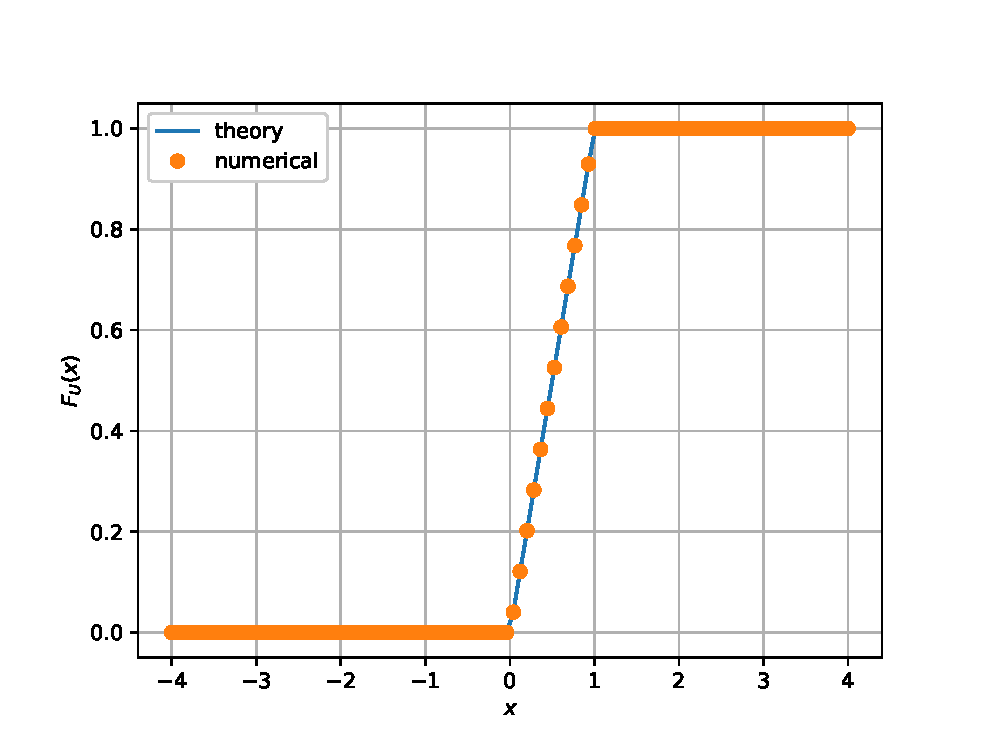
\includegraphics[scale = 0.6]{./figs/uni_cdf} \label{fig:uni_cdf}
        \caption{CDF of U}
        \end{figure}

\item Find a theoretical expression for $F_U(x)$.\\

\solution Since We have,
    
    \begin{align}
    P_U(x) =  \begin{cases}
        \frac{1}{b-a} & x \in (a,b) \\
        0 & otherwise
    \end{cases} 
    \end{align}

    on integrating for CDF we get,
    
    \begin{align}
    F_U(x) =  \begin{cases}
        \frac{x-a}{b-a} & x \in (a,b) \\
        0 & otherwise
    \end{cases} 
    \end{align}

    Here, we have a=0 and b=1, Hence,
    
    \begin{align}
    F_U(x) =  \begin{cases}
        x& x \in (0.1) \\
        0 & otherwise
    \end{cases} 
\end{align}

\item Write a C program to find the mean and variance of U.\\

\solution download C program

\begin{lstlisting}
$ wget https://raw.githubusercontent.com/galaxion-tech/AI1110/master/ass_manual/prob1.4/mycode1.c
        \end{lstlisting}
        and compiled and executed with
        \begin{lstlisting}
$ gcc mycode1.c -lm -Wall -g
$ ./a.out
        \end{lstlisting}
    \begin{align}
        E[U] &= 0.500007  \label{eq:1.4.1}\\
        \text{Var}[U] &= 0.083301 \label{eq:1.4.2}
    \end{align}
\item Verify your result theoretically given that 
    \begin{equation}
        E[U^k] = \int_{- \infty}^{\infty} x^k dF_U(x)
    \end{equation}
    \solution we have 
    \begin{align}
        E[U] &= \int_{-\infty}^{\infty} xdF_U(x) \\
        &= \int_{0}^1 x dx \\
        &=  0.5
    \end{align}
    From \eqref{eq:1.4.1}, we have, 
    \begin{equation}
        E[U] = 0.500007 \approx 0.5
    \end{equation}
    Similarly,
    \begin{align}
        \text{Var}[U]&=E[U^2]-(E[U])^2 \\
        &=\int_{-\infty}^{\infty}x^2dF_U(x) - 0.25\\
        &=\int_{0}^{1}x^2dx - 0.25\\
        &=0.3333...-0.25=0.083333...
    \end{align}
    From \eqref{eq:1.4.2},we get
    \begin{equation}
        \text{Var}[U] = 0.083301 \approx 0.08333..
    \end{equation}
    Hence Verified.
\end{enumerate}
\section{Central Limit Theorem}
\begin{enumerate}[label=\thesection.\arabic*.,ref=\thesection.\theenumi]
\numberwithin{equation}{enumi}
\numberwithin{figure}{enumi}
\numberwithin{table}{enumi}


\item Generate $10^6$ samples of the random variable
    \begin{equation}
        X=\sum_{i=1}^{12} U_i-6        
    \end{equation}
    using a C program, where $U_i, i = 1, 2,\ldots, 12$ are a set of independent uniform random variables between 0 and 1 and save in a file called gau.dat.\\
    
    
    \solution Download the file

    \begin{lstlisting}    
$ wget https://raw.githubusercontent.com/galaxion-tech/AI1110/master/ass_manual/prob2.1/mycode2.c
    \end{lstlisting}

    Use coeffs.h from the prob1.1\\
    And run the code as:

    \begin{lstlisting}
$ gcc mycode2.c -lm -Wall -g
$ ./a.out
\end{lstlisting}

\item Load gau.dat in python and plot the empirical CDF of $X$ using the samples in gau.dat. What properties does a CDF have?\\

\solution 
    The required python file can be downloaded using

    \begin{lstlisting}
 $ wget https://raw.githubusercontent.com/galaxion-tech/AI1110/master/ass_manual/prob2.2/mycode3.py
\end{lstlisting}

and executed using

\begin{lstlisting}
$ python3 mycode3.py
\end{lstlisting}

Graph is as follow:
    \begin{figure}[H]
        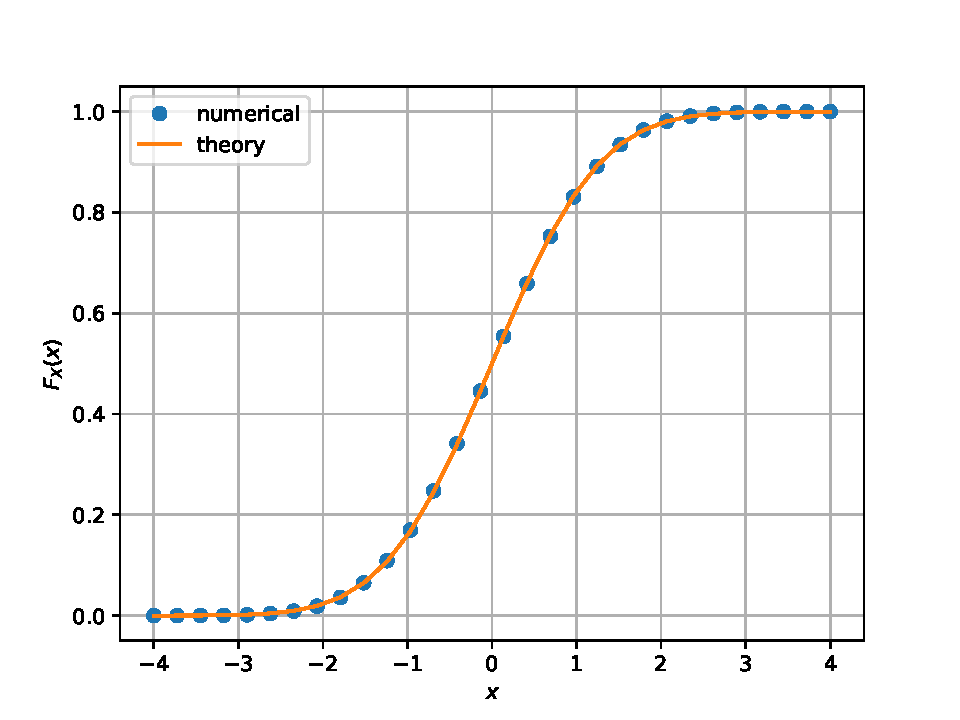
\includegraphics[scale=0.6]{./figs/gau_cdf}
        \caption{CDF of X}
    \end{figure}

    CDF has properties:
    \begin{itemize}
        \item CDF is non-decreasing
        \item $\lim_{x \leftarrow -\infty} F_X(x) = 0 $
        \item $ \lim_{x \leftarrow \infty} F_X(x) = 1 $
        \item It is right continous
    \end{itemize}


    \item Load gau.dat in python and plot the empirical PDF of X using the samples in gau.dat. The PDF of X is defined as
    \begin{equation}
        P_X(x) = \frac{d}{dx}F_X(x)
    \end{equation}
    What properties does the PDF have?\\

    \solution 
    The required python file can be downloaded using

    \begin{lstlisting}
 $ wget https://raw.githubusercontent.com/galaxion-tech/AI1110/master/ass_manual/prob2.3/pdf_plot.py
\end{lstlisting}

and executed using

\begin{lstlisting}
$ python3 pdf_plot.py
\end{lstlisting}

Graph is as follow:
    \begin{figure}[H]
        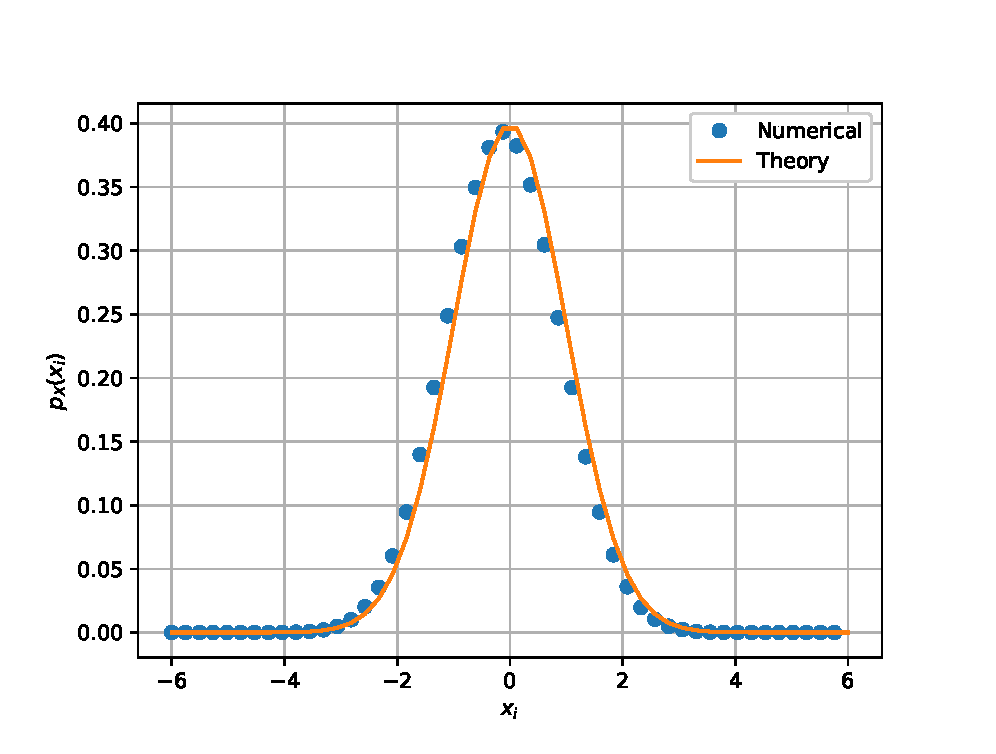
\includegraphics[scale=0.6]{./figs/gauss_pdf}
        \caption{PDF of X}
    \end{figure}

    PDF has properties: 
    \begin{itemize}
        \item $\int_{-\infty}^{\infty} P_X(x) dx = 1$
        \item $\forall x \in \mathbb{R} \hspace{12pt} P_X(x) \leq 0$
        \item $\forall a<b \hspace{12pt} a,b \in \mathbb{R} \\ Pr(a<x<b) = Pr(a\leq x\leq b) = \int_a^b P_X(x) dx$
    \end{itemize}


    \item Find the mean and variance of X by writing a C program.\\

    \solution 

\noindent The C program can be downloaded using

\begin{lstlisting}
$ wget https://raw.githubusercontent.com/galaxion-tech/AI1110/master/ass_manual/prob2.4/mycode4.c
\end{lstlisting}

and compiled and executed with the following commands

\begin{lstlisting}
$ gcc mycode4.c -lm -Wall -g
$ ./a.out
\end{lstlisting} 

On running, we get
    \begin{align}
        E[X] = 0.000326 \\
        \text{Var}[X] = 1.000907
    \end{align}


    \item Given that
     \begin{equation}
        P_X(x) = \frac{1}{\sqrt{2\pi}}\text{exp}\left(\frac{-x^2}{2}\right), -\infty < x < \infty
     \end{equation}
     Find Mean and Varaince theoretically.\\
     \solution we have,
     \begin{align}
        E[X] &= \int_{-\infty}^{\infty}xP_X(x)dx \\
        &= \int_{-\infty}^{\infty}x\frac{1}{\sqrt{2\pi}}e^{\frac{-x^2}{2}}dx \\
        &=\left. \frac{1}{\sqrt{2\pi}}(-e^{\frac{-x^2}{2}}) \right|_{x=-\infty}^{x=\infty}\\
        &=0
     \end{align}
     \begin{align}
        \text{Var}[X]&=E[X^2]-(E[X])^2 \\
        &=\int_{-\infty}^{\infty}x^2P_x(x)dx \\
        &=\int_{-\infty}^{\infty}x^2\frac{1}{\sqrt{2\pi}}e^{\frac{-x^2}{2}}dx \\
        &=\int_{-\infty}^{\infty}\frac{1}{\sqrt{2\pi}}e^{\frac{-x^2}{2}}dx\\
        &=\int_{-\infty}^{\infty}P_X(x)dx\\
        &=1
     \end{align}
\end{enumerate}
\section{From Uniform to other}
\begin{enumerate}[label=\thesection.\arabic*.,ref=\thesection.\theenumi]
\numberwithin{equation}{enumi}
\numberwithin{figure}{enumi}
\numberwithin{table}{enumi}

\item Generate samples of
\begin{equation}
    V = -2 \ln (1-U)
\end{equation}
and plot its CDF.\\
\solution 

Download the C code to create the distribution.

\begin{lstlisting}
$ wget https://raw.githubusercontent.com/galaxion-tech/AI1110/master/ass_manual/prob3.1/mycode6.c
\end{lstlisting}
and can be executed with
\begin{lstlisting}
$ gcc mycode6.c -lm -Wall -g
$ ./a.out
\end{lstlisting}

The relevant python code is at

\begin{lstlisting}
 $ wget https://raw.githubusercontent.com/galaxion-tech/AI1110/master/ass_manual/prob3.1/mycode5.py
\end{lstlisting}
and can be executed with
\begin{lstlisting}
$ python3 mycode5.py
\end{lstlisting}

CDF Graph is as follow 
\begin{figure}[H]
    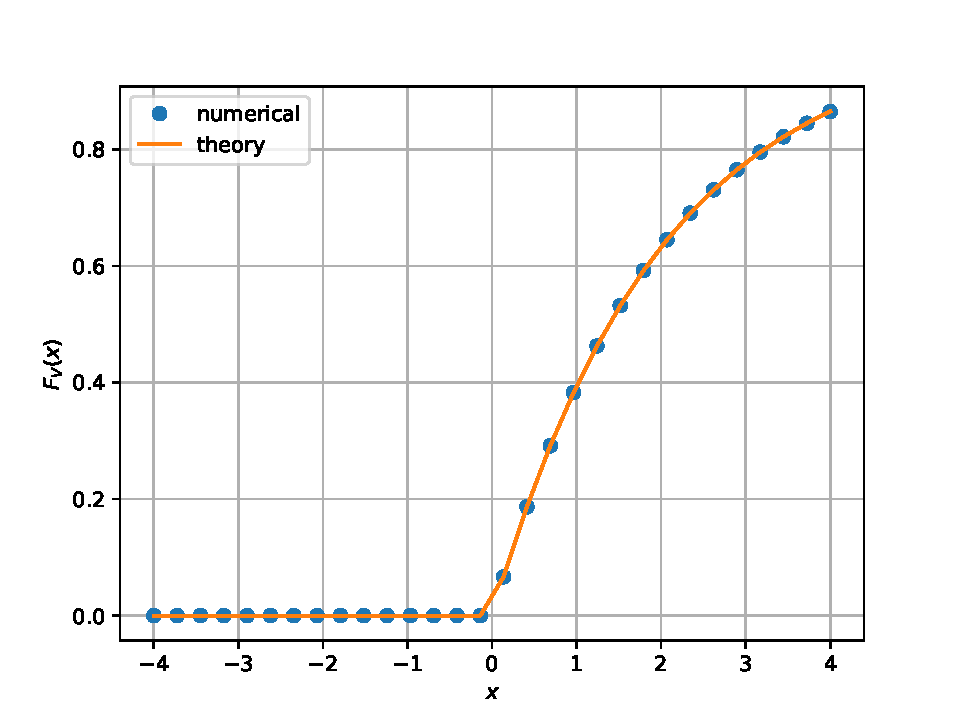
\includegraphics[scale=0.6]{./figs/other_cdf}
    \caption{CDF of V}
\end{figure}

\item Find a theoretical expression for $F_V (x)$.\\
\solution 
    \begin{align}
        F_V(x) &= Pr(V<x)\\
        &= Pr(-2\ln(1-U) < x)\\
        &= Pr(U<1-e^{\frac{-x}{2}}) \\
        &= F_U(1-e^{\frac{-x}{2}})
    \end{align}
    Therfore,
    \begin{align}
        F_V(x) = \begin{cases}
        0 & x \in (-\infty,0] \\
        1-e^{\frac{-x}{2}} & x \in (0,\infty)
    \end{cases} 
    \end{align}
\end{enumerate}

\end{document}